\documentclass{article}

\usepackage{multicol}
\usepackage{graphicx}
\usepackage{float}
\usepackage{listings}
\usepackage{dirtytalk}
\usepackage{amsmath}
\usepackage{hyperref}
\usepackage{smartref}
\usepackage{svg}
\usepackage{textgreek}
\usepackage[a4paper,margin=2cm]{geometry}

\lstset{basicstyle=\ttfamily\footnotesize,breaklines=true}

\title{DSP Assignment 3 \\ \textit{Wireless Data Transmission Using Lasers}}
\author{Amana Ahmmad, Logan Brown \\ 2590941A, 2641407B}

\begin{document}
\maketitle

\begin{multicols}{2}

\section{Introduction}
Data are usually transmitted wirelessly using sub-infrared frequencies: radio waves, microwaves, and so on. Transmission is usually performed using an omni-directional antenna - this is desirable as the transmitter need not know where the receiver is relative to itself.  

However, there exist use cases where the transmitter may not want to send its data in all directions. If the receiver and transmitter are stationary and in known locations, but it is for some reason not practicable to lay cable between the two, a highly directional wireless system may be more ideal. 

In this case, using a laser to send the data, rather than an antenna, is a possibility. This report explores the use of a laser diode to send data, in conjunction with a phototransistor to detect the signal.

\section{Data framing}
Since the receiver and transmitter are separated, there cannot be a clock line between the two, necessitating the use of an asynchronous scheme. 

To frame the data, UART (universal asynchronous receiver-transmitter) was chosen, as it is commonly used, well documented, and well tested. Python code was written to emulate a UART transmitter (Tx) and receiver (Rx), with two classes that would output 0 or 1, or read 0 or 1 respectively.

The \texttt{UART\_Tx} class allows the user to load an array of bytes, which are then \say{sent} automatically. The \texttt{UART\_Rx} class constantly listens for changes at 8 times the baud rate, and outputs a byte as soon as it determines that it has received one.

\section{Set up}
The laser was aimed at a phototransistor which was set up in a voltage-divider configuration, as outlined in Figure \ref{fig:circuit},\ref{fig:dataflow}. An Arduino connected to a computer measured the voltage across the resistor. As only one Arduino was available, the same device sent the signal as received it, though the setup would work equally with two separate devices. 

An FSK modulation scheme was used. A logic 0 corresponds to the laser being switched off, effectively 0 Hz, while a logic 1 corresponds to the laser being keyed on and off at a given frequency. This was chosen to be 100 Hz, as it would be significantly higher than any environmental optical and electronic noise, but low enough that it can be reliably sampled at 1000 Hz with minimal aliasing.

\begin{figure}[H]
    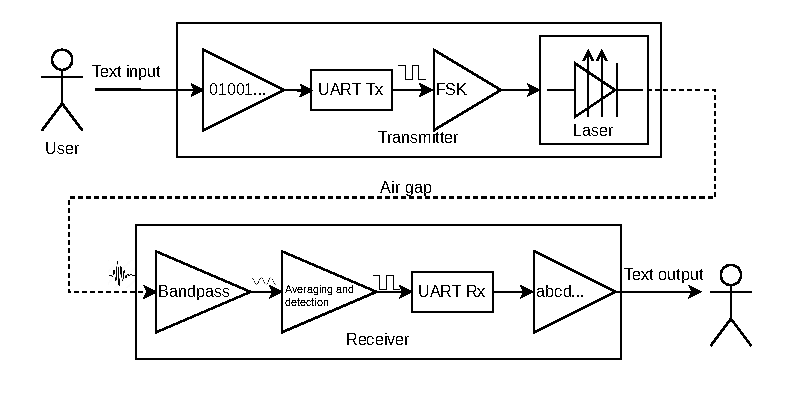
\includegraphics[width=\linewidth]{figures/dataflow.pdf}
    \caption{Dataflow diagram}
    \label{fig:dataflow}
\end{figure}

\begin{figure}[H]
    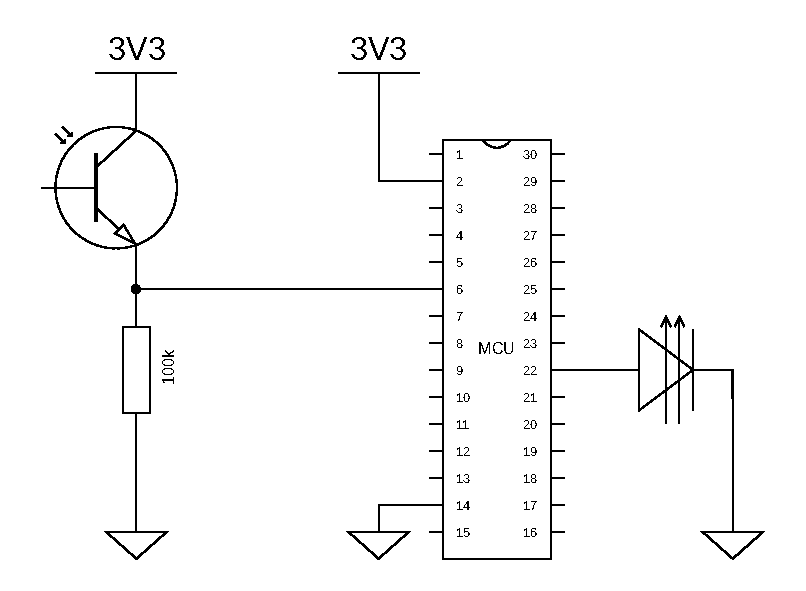
\includegraphics[width=\linewidth]{figures/circuit.pdf}
    \caption{Circuit diagram}
    \label{fig:circuit}
\end{figure}

\section{Filtering}
The phototransistor has a relatively wide wavelength response, peaking in near-infrared but extending into shorter-wavelength visible light, and longer infrared. Thus, it responds to much of the ambient light in an environment, and so there is a significant amount of noise in the signal -- both optical and electrical.

The main sources of noise are the 50 Hz mains electric hum, very low-frequency drift from natural sources, and DC drift from the ambient light level. 

To remove these unwanted frequencies, an 8\textsuperscript{th} order (or rather, a chain of 4 2\textsuperscript{nd} order) bandpass IIR filter was used, with the passband being 5 Hz either side of the sending frequency. 

\section{Other processing}
The output of a narrow bandpass filter centered on the fundamental frequency of a square wave will inevitably be a sine wave, since it will discard all harmonics of the square wave (indeed, this can be seen in the filtered data in Figure \ref{fig:filtered}). To turn this sine wave into a low or high digital signal, some additional processing was required. 

This involved taking the mean of the last 2 cycles of the wave. The mean of a sine wave is always 0, so first the absolute value of the data was taken, then averaged. This resulted in a fairly steady high or low value. A static threshold was used to determine whether the value constituted a logic high or logic low.

\section{Baud rate}
Finally, the baud rate of the UARTs was set to 10. The delay of the IIR filter and the response of the phototransistor were slow enough that sending faster than this would not allow the logic levels enough time to settle, resulting in missed bits. Naturally, this would be too slow for a real world scenario, but with more research and engineering it would be relatively trivial to make this faster. 

\section{Sampling}
Sampling was performed using an Arduino running \textit{pyFirmata2}. This involves using a callback function in Python, which is run periodically at a fixed interval. 

To ensure that the sampling was correct, the time taken for the callback to run was measured and stored. The results of this are in Figure \ref{fig:sampling}. 

If the time taken for the sampling callback exceeds the sampling period, the actual sampling rate will decrease. If the filtering is happening with an assumed sampling rate of 1 kHz, with frequencies warped with this assumption, then the frequencies perceived in the data will be incorrect, leading to poor filter performance.

Rather than have all the filtering and processing happen in the callback, the callback appended the data to a thread-safe queue, and a separate function was called every 10 milliseconds which would take the data from the queue and process it. Since there is a certain amount of context switching overhead involved with swapping between threads, running a longer computation less often leads to better performance, provided (as is the case here) that the buffering of data is not to the detriment of other parts of the program. 

\section{Results and discussion}
\begin{figure}[H]
    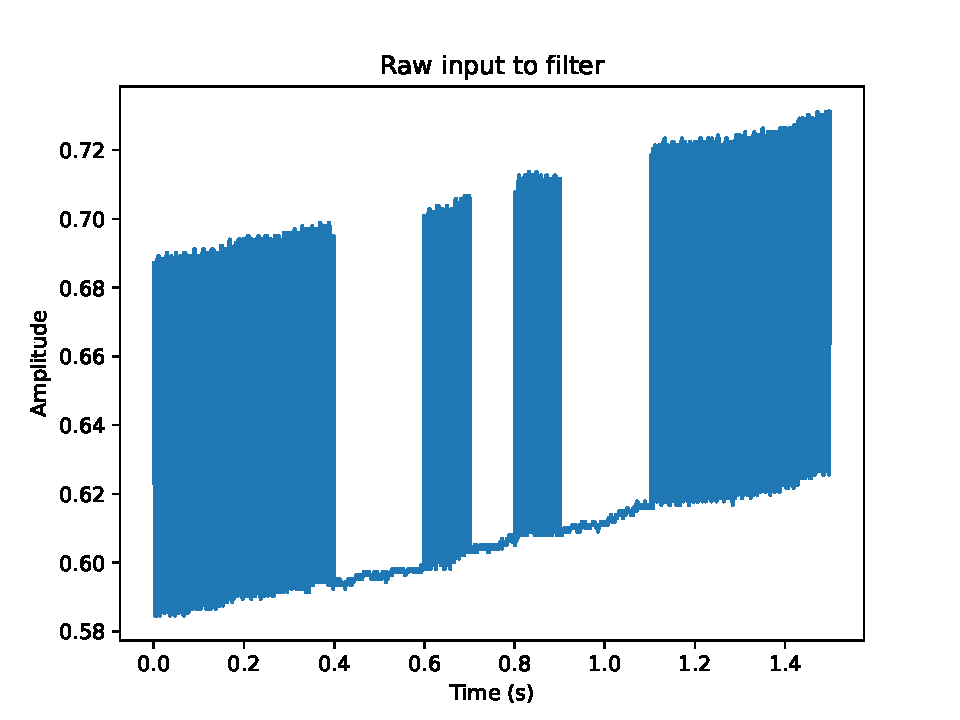
\includegraphics[width=\linewidth]{figures/raw.pdf}
    \caption{Raw, unfiltered data from analogue input}
    \label{fig:raw}
\end{figure}

\begin{figure}[H]
    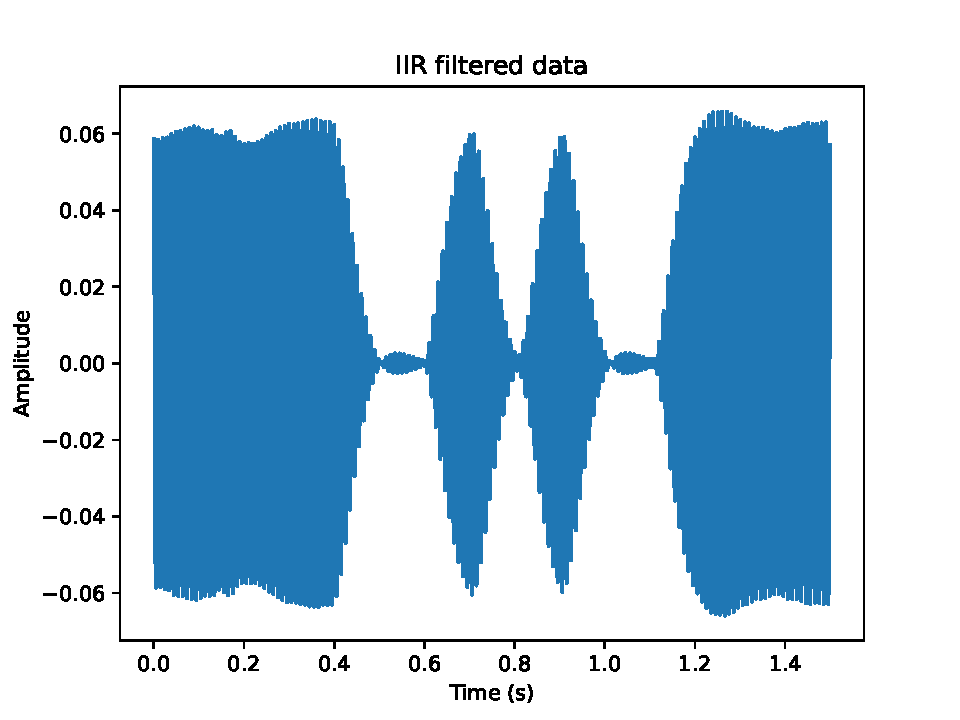
\includegraphics[width=\linewidth]{figures/filtered.pdf}
    \caption{Data filtered using a bandpass IIR filter}
    \label{fig:filtered}
\end{figure}

\begin{figure}[H]
    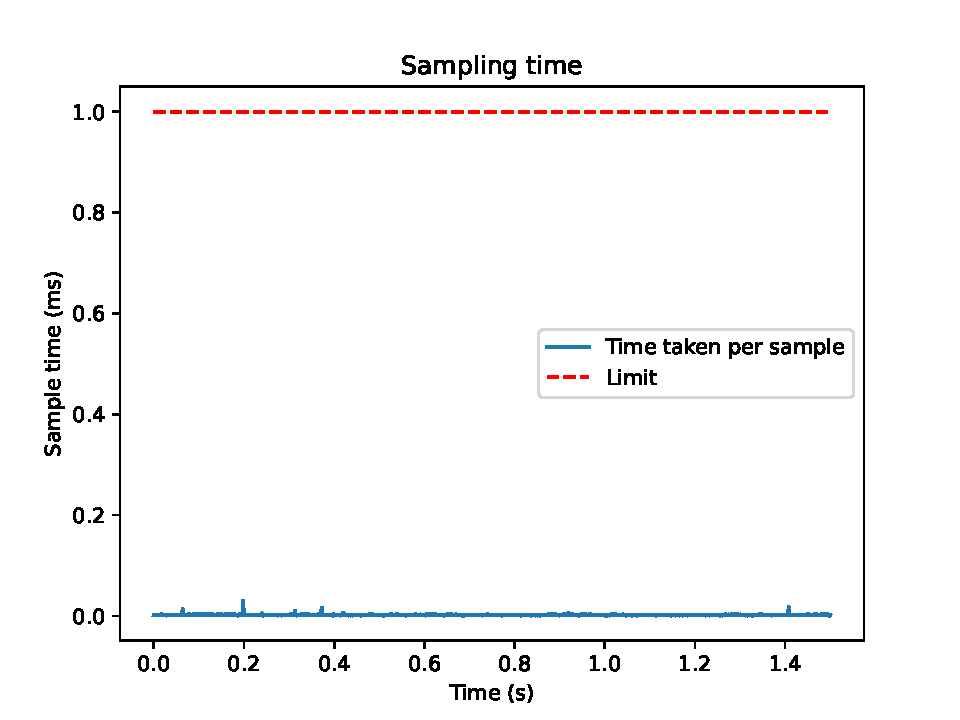
\includegraphics[width=\linewidth]{figures/sampling.pdf}
    \caption{Time taken per sample}
    \label{fig:sampling}
\end{figure}

\begin{figure}[H]
    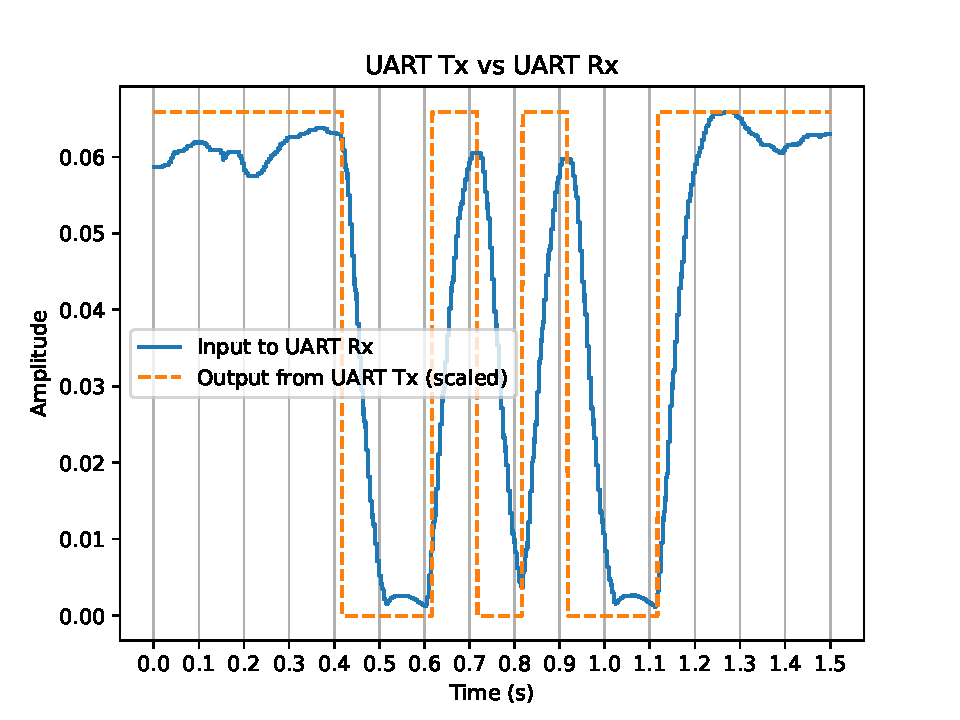
\includegraphics[width=\linewidth]{figures/uart.pdf}
    \caption{Output from UART transmitter, versus input to UART receiver}
    \label{fig:uart}
\end{figure}

As can be seen from Figure \ref{fig:raw}, there was a significant DC offset and drift in the raw data. This is entirely eliminated in Figure \ref{fig:filtered}, demonstrating the performance of the IIR filter. Unfortunately, the filter was not as responsive as one might hope, causing the lobing effect that can be seen in the plot. This delay can also be seen in Figure \ref{fig:uart}. 

Figure \ref{fig:uart} shows how the transmitter sent its data (in this case, the letter \say{S}), and how the receiver saw that data. Marked on the plot are the bits of the UART frame.

While it was important to measure the callback time, it can be seen from Figure \ref{fig:sampling} that the time taken was always far below the limit of 1 ms, with the longest period being just 30 \textmu s.

To test the accuracy, a 128 byte message was sent (taking 141 seconds). Across 5 runs, the mean accuracy (i.e. the number of correct bits divided by the number of bits in the message) was 0.972. This could be increased by using a parity bit, but this would require at least half-duplex, as the receiver would have to have a mechanism for requesting retransmission of dropped frames. 

\section{Conclusion}
It was possible to send large amounts of data with very little loss, albeit quite slowly. The IIR filter performed well, eliminating all environmental noise and providing a clean signal to the UART receiver, though there was a significant delay in the response that limited the baud rate.

Some potential improvements may involve: increasing the accuracy with parity bit(s); increasing the number of sending frequencies to increase the bits per symbol beyond 1; quickening the response of the filtering; or adding a mechanism to automatically choose a threshold, rather than manually setting it.  

\end{multicols}
\pagebreak

\section{Appendix}
A video showing the realtime filtering can be found here: \href{https://youtu.be/iLDZ0yH2ANQ}{https://youtu.be/iLDZ0yH2ANQ}

\subsection{uart.py}
\lstinputlisting[language=python]{../python/uart.py}

\subsection{filter.py}
\lstinputlisting[language=python]{../python/filter.py}

\subsection{graph.py}
\lstinputlisting[language=python]{../python/graph.py}

\subsection{receiver.py}
\lstinputlisting[language=python]{../python/receiver.py}

\subsection{transmitter.py}
\lstinputlisting[language=python]{../python/transmitter.py}

\subsection{config.py}
\lstinputlisting[language=python]{../python/config.py}


\end{document}